\documentclass[12pt]{article}
\usepackage[margin=1in]{geometry}
\usepackage{graphicx}
\usepackage{amsmath}
\usepackage{hyperref}
\usepackage{appendix}

% Python listing setup

\usepackage{color}
\usepackage[procnames]{listings}
\usepackage{textcomp}
\usepackage{setspace}
\renewcommand{\lstlistlistingname}{Code Listings}
\renewcommand{\lstlistingname}{Code Listing}
\renewcommand{\ttdefault}{pcr}
\definecolor{gray}{gray}{0.5}
\definecolor{green}{rgb}{0,0.5,0}
\definecolor{brown}{rgb}{0.5,0.25,0}
\definecolor{lightgreen}{rgb}{0,0.7,0}
\definecolor{darkgreen}{rgb}{0,0.4,0}
\definecolor{purple}{rgb}{0.5,0,0.5}
\definecolor{darkred}{rgb}{0.5,0,0}
\lstnewenvironment{python}[1][]{
\lstset{
language=python,
basicstyle=\ttfamily\small\setstretch{1},
stringstyle=\color{brown},
showstringspaces=false,
alsoletter={1234567890},
otherkeywords={\ , \}, \{},
keywordstyle=\color{blue},
emph={access,and,as,break,class,continue,def,del,elif,else,%
except,exec,finally,for,from,global,if,import,in,is,%
lambda,not,or,pass,print,raise,return,try,while,assert},
emphstyle=\color{darkgreen}\bfseries,
emph={[2]self},
emphstyle=[2]\color{gray},
emph={[4]ArithmeticError,AssertionError,AttributeError,BaseException,%
DeprecationWarning,EOFError,Ellipsis,EnvironmentError,Exception,%
False,FloatingPointError,FutureWarning,GeneratorExit,IOError,%
ImportError,ImportWarning,IndentationError,IndexError,KeyError,%
KeyboardInterrupt,LookupError,MemoryError,NameError,None,%
NotImplemented,NotImplementedError,OSError,OverflowError,%
PendingDeprecationWarning,ReferenceError,RuntimeError,RuntimeWarning,%
StandardError,StopIteration,SyntaxError,SyntaxWarning,SystemError,%
SystemExit,TabError,True,TypeError,UnboundLocalError,UnicodeDecodeError,%
UnicodeEncodeError,UnicodeError,UnicodeTranslateError,UnicodeWarning,%
UserWarning,ValueError,Warning,ZeroDivisionError,abs,all,any,apply,%
basestring,bool,buffer,callable,chr,classmethod,cmp,coerce,compile,%
complex,copyright,credits,delattr,dict,dir,divmod,enumerate,eval,%
execfile,exit,file,filter,float,frozenset,getattr,globals,hasattr,%
hash,help,hex,id,input,int,intern,isinstance,issubclass,iter,len,%
license,list,locals,long,map,max,min,object,oct,open,ord,pow,property,%
quit,range,raw_input,reduce,reload,repr,reversed,round,set,setattr,%
slice,sorted,staticmethod,str,sum,super,tuple,type,unichr,unicode,%
vars,xrange,zip},
emphstyle=[4]\color{purple}\bfseries,
upquote=true,
morecomment=[s][\color{lightgreen}]{"""}{"""},
commentstyle=\color{red}\slshape,
literate={>>>}{\textbf{\textcolor{darkred}{>{>}>}}}3%
         {...}{{\textcolor{gray}{...}}}3,
procnamekeys={def,class},
procnamestyle=\color{blue}\textbf,
framexleftmargin=1mm, framextopmargin=1mm,
rulesepcolor=\color{blue},#1
}
}{}


\title{\huge \bf Track-Based Alignment Tutorial}
\author{Jim Pivarski}

\begin{document}
\maketitle

\section{Introduction}
\label{sec:introduction}

Tracking detectors are designed to record the trajectories of charged
particles with as much precision as possible, but if the location of a
detector is not precisely known, then neither are the tracks it
reports.  The situation is even worse when a tracking system is
composed of many subdetectors and each is imprecisely positioned
relative to the others: smoothly-curving trajectories would appear to
be erratic, and parameters of track-fits would be inaccurate.  To
``align'' a tracking system is to correct this situation, not
necessarily by physically moving the subdetectors into a specified
configuration, but by precisely measuring the as-built positions and
orientations of all subcomponents and supplying the information to
track-fitting algorithms for better reconstruction.

\begin{center}
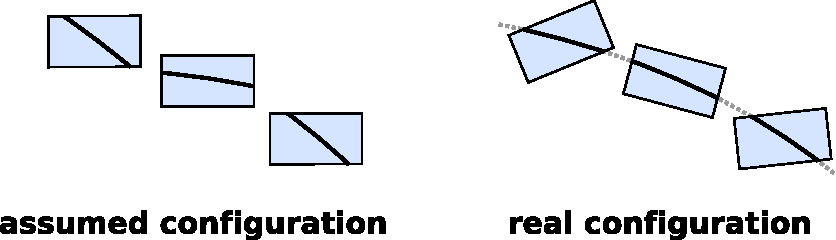
\includegraphics[width=0.65\linewidth]{PLOTS/why_alignment_is_important.pdf}
\end{center}

There are many ways to measure the position of an object, but a
particularly natural way to measure the position of a tracking
detector is to use the tracks themselves.  Tracking detectors are
complicated objects with active (particle-sensing) components
surrounded by support structures, often sealed to contain an ionizable
gas.  It can sometimes be difficult to relate measurements of the
outside of the detector to the positions of the active components
inside.  The charged particles, however, are directly observed by the
active elements, so if the trajectories of the particles could be
known, then they would provide a position measurement of the important part
of the detector.

This may sound like a circular argument: measure chamber positions
with particle trajectories, and then measure particle trajectories
with respect to the known chamber positions.  The circularity is
resolved by the fact that we know how particles propagate through
space, at least in a statistical sense for an ensemble of tracks.  For
example, if all tracks passing through two subdetectors appear to
deviate from extrapolated trajectories by the same offset
somewhere between the subdetectors, then we can assume that the
subdetectors are misaligned by the value of that offset.  The
difficult task is to understand the propagation of particles in
detail, so that the average of extrapolations from one subdetector to
another is statistically precise and free of bias, to a given level of
accuracy.

\begin{center}
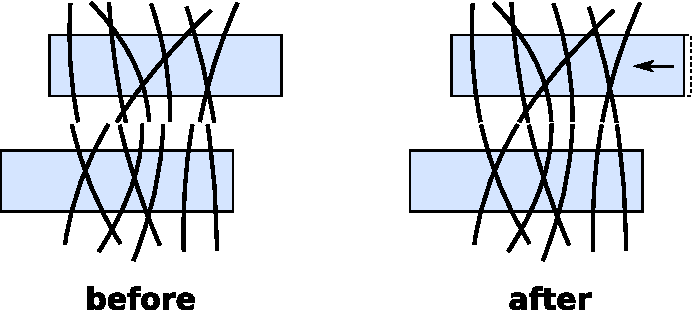
\includegraphics[width=0.6\linewidth]{PLOTS/alignment_with_tracks.pdf}
\end{center}

This note describes the central concepts of track-based alignment with
toy examples and illustrations drawn from the alignment of the CMS muon
system.  It is a pedagogical text, rather than a how-to manual, to
help the reader develop expertise in thinking about and solving
alignment problems.  The toy examples are open-ended to allow the
reader to ``tinker'' with simplified alignment systems.  Some
familiarity with the Python scripting language is assumed, and the
following software packages are required:
\begin{itemize}
\item Python \href{http://python.org/}{\tt http://python.org/};
\item NumPy \href{http://numpy.scipy.org/}{\tt http://numpy.scipy.org/} for linear algebra;
\item PyMinuit \href{http://code.google.com/p/pyminuit/}{\tt http://code.google.com/p/pyminuit/} for non-linear
  minimization;
\item pyROOT \href{http://root.cern.ch/}{\tt http://root.cern.ch/} for plotting.
\end{itemize}
Not all packages are required for all examples, and other tools that
provide the same functionality could be substituted if desired.

The note covers three major topics: combining alignment measurements,
measuring detector positions with tracks, and investigating track
biases.  The first is covered in
section~\ref{sec:propagating_alignment_measurements}, which explains
how relative measurements of subdetectors can be combined into a
mutually consistent system, and how to propagate uncertainties through
complex networks of inter-alignments.
Section~\ref{sec:measuring_detector_positions_with_tracks} shows how
trends in tracking distributions can be used to measure the position
and orientation of a detector.  In
section~\ref{sec:realistic_tracking_and_diagnostics_of_track_bias},
common biases in track distributions are discussed with methods of
diagnosing data from a tracking system.  Finally,
section~\ref{sec:cscoverlapsalignmentalgorithm_a_complete_alignment_package}
presents a configurable alignment package in CMSSW, so that alignment
concepts can be applied in a real setting.

\section{Propagating Alignment Measurements}
\label{sec:propagating_alignment_measurements}

Suppose that the positions of $N_a$ alignable objects are related to
one another by $N_m$ measurements.  How can these data be combined
into a single configuration?  Can such a configuration be internally
consistent, given measurement uncertainties?  How can measurement
uncertainties be propagated to uncertainties in the positions of the
aligned system?  This section covers the problem of deriving a global
alignment configuration from relative measurements between alignable
objects, a topic not restricted to track-based alignment.  All
alignment problems in this section are one-dimensional but with many
objects to be aligned in that dimension;
section~\ref{sec:measuring_detector_positions_with_tracks} covers
multi-dimensional problems, but usually with only one alignable object
for simplicity.

\subsection{Motivating examples}

\vspace{0.2 cm}
\begin{minipage}{\linewidth}
We'll start with a simple case: $N_a=5$ alignables $A_i$ with $N_m=4$
one-dimensional measurements $m_{i,i+1}$ of the displacement between
neighbors.
\begin{center}
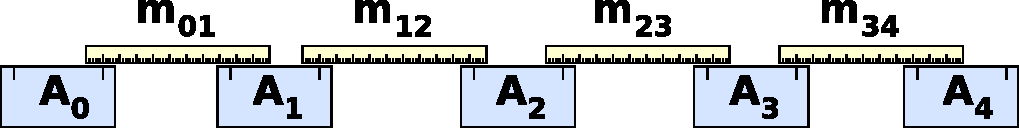
\includegraphics[width=0.8\linewidth]{PLOTS/propagating_example1.pdf}
\end{center}
\end{minipage}

\vspace{0.4 cm}
We want to describe the positions of all $A_i$ from the measurements.
The first issue is that a global coordinate system has not been
defined in which to express the solution, and even if an external
coordinate system were to be provided, there would be no way to relate
$A_i$ to the origin of that system without an additional measurement.
Providing both an external coordinate system and a measurement between
it and the first or last alignable reduces the problem to what we had
before, with its origin as a new $A_i$ and the measurement as a new
$m_{i,i+1}$.  It is therefore equivalent to choose one of the $A_i$ as
the origin of the coordinate system.  We could say that $A_0=0$ by
definition.

Now we can solve the problem easily:
\begin{equation}
\begin{array}{r c l}
A_1 & = & m_{01} \\
A_2 & = & m_{01} + m_{12} \\
A_3 & = & m_{01} + m_{12} + m_{23} \\
A_4 & = & m_{01} + m_{12} + m_{23} + m_{34}.
\end{array}
\label{eqn:propagating_example1}
\end{equation}
Where did this result come from?  We intuitively solved the following
system of equations:
\begin{equation}
\begin{array}{r c l}
A_0 &=& 0 \\
m_{01} &=& A_1 - A_0 \\
m_{12} &=& A_2 - A_1 \\
m_{23} &=& A_3 - A_2 \\
m_{34} &=& A_4 - A_3.
\end{array}
\label{eqn:propagating_example2}
\end{equation}

Now suppose that we want to know the uncertainty in $A_4$, given
uncertainties in the measurements $\sigma_{i,i+1}$.  Applying the
standard error propagation formula to
Eq.~\ref{eqn:propagating_example1}, the uncertainty in $A_4$ is
\begin{equation}
\sqrt{{\sigma_{01}}^2 + {\sigma_{12}}^2 + {\sigma_{23}}^2 + {\sigma_{34}}^2}.
\end{equation}
Clearly, the uncertainty in $A_4$ must be larger than the uncertainty
in any other alignable, but this is simply due to our choice of
coordinate system.  If we had chosen $A_3$ as the origin, then the
uncertainty in $A_4$ would be only $\sigma_{34}$, and if we had chosen
$A_4$ as the origin, then the uncertainty would be zero.  Moreover,
there are strong correlations between $A_3$ and $A_4$, because if
$m_{23}$ fluctuates up by some amount, then $A_3$ and $A_4$ both
fluctuate up together.  Independent measurements do not result in
independent alignment positions.

\vspace{0.2 cm}
\noindent \begin{minipage}{\linewidth}
\hspace{0.4 cm} Let's add a little to our example by closing the loop: a new
measurement $m_{40}$ directly relates the position of $A_4$ to that of
$A_0$.
\begin{center}
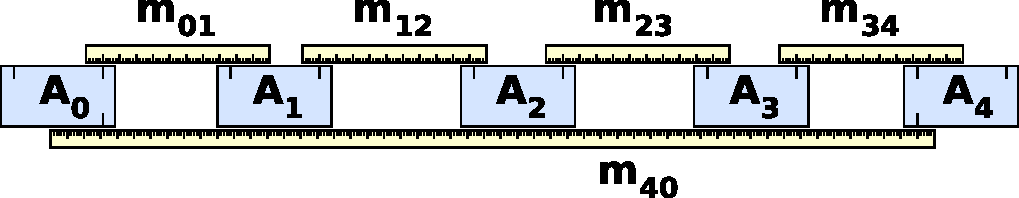
\includegraphics[width=0.8\linewidth]{PLOTS/propagating_example3.pdf}
\end{center}
\end{minipage}

If we propagate the information about the system as we did before, we
might find that the new measurement is incompatible with the first
four: $m_{40} \ne m_{01} + m_{12} + m_{23} + m_{34}$, possibly due to
a statistical error, or possibly due to a mistake in the measurments.
How do we solve the system now?  $A_4 = m_{01} + m_{12} + m_{23} +
m_{34}$ yields a different result than $A_4 = -m_{40}$, so which do we
choose?

The new system is overconstrained, so in general we cannot find a
solution that satisfies all measurements exactly.  However, we can
find a set of $A_i$ that is the best fit to $m_{i,i+1}$ by minimizing
an objective function like
\begin{multline}
\chi^2 = (A_0)^2 + (m_{01} - A_1 + A_0)^2 + (m_{12} - A_2 + A_1)^2 + \\
 (m_{23} - A_3 + A_2)^2 + (m_{34} - A_4 + A_3)^2 + (m_{40} - A_0 + A_4)^2.
\end{multline}
In the minimization, we are asking for $A_{i+1} - A_i$ to be as close
as possible to $m_{i,i+1}$ for all measurements simultaneously, and
for $A_0$ to be as close as possible to zero (compare with
Eq.~\ref{eqn:propagating_example2}).  The function can be minimized
analytically:
\begin{equation}
\begin{array}{r c r c l}
\displaystyle \frac{1}{2} \frac{\partial \chi^2}{\partial A_0} &=& A_0 + (-1) (m_{40} - A_0 + A_4) + (1) (m_{01} - A_1 + A_0) &=& 0 \vspace{0.2 cm} \\
\displaystyle \frac{1}{2} \frac{\partial \chi^2}{\partial A_1} &=& (-1) (m_{01} - A_1 + A_0) + (1) (m_{12} - A_2 + A_1) &=& 0 \vspace{0.2 cm} \\
\displaystyle \frac{1}{2} \frac{\partial \chi^2}{\partial A_2} &=& (-1) (m_{12} - A_2 + A_1) + (1) (m_{23} - A_3 + A_2) &=& 0 \vspace{0.2 cm} \\
\displaystyle \frac{1}{2} \frac{\partial \chi^2}{\partial A_3} &=& (-1) (m_{23} - A_3 + A_2) + (1) (m_{34} - A_4 + A_3) &=& 0 \vspace{0.2 cm} \\
\displaystyle \frac{1}{2} \frac{\partial \chi^2}{\partial A_4} &=& (-1) (m_{34} - A_4 + A_3) + (1) (m_{40} - A_0 + A_4) &=& 0.
\end{array}
\end{equation}
Rearranging it and casting it in matrix form, the problem becomes
\begin{equation}
\left(\begin{array}{c}
m_{40} - m_{01} \\
m_{01} - m_{12} \\
m_{12} - m_{23} \\
m_{23} - m_{34} \\
m_{34} - m_{40} \\
\end{array}\right) = \left(\begin{array}{r r r r r}
1 + 2 & -1 & 0 & 0 & -1 \\
-1 & 2 & -1 & 0 & 0 \\
0 & -1 & 2 & -1 & 0 \\
0 & 0 & -1 & 2 & -1 \\
-1 & 0 & 0 & -1 & 2 \\
\end{array}\right) \left(\begin{array}{c}
A_0 \\
A_1 \\
A_2 \\
A_3 \\
A_4 \\
\end{array}\right) \mbox{ or } \vec{v} = M \cdot \vec{A},
\label{eqn:propagating_example3}
\end{equation}
which can be solved by matrix inversion: $\vec{A} = M^{-1} \cdot \vec{v}$.

If $m_{40} \ne m_{01} + m_{12} + m_{23} + m_{34}$, the matrix solution
spreads non-zero values of $m_{i,+1} - A_{i+1} + A_i$ (the
``fit residuals'') equally among all alignables.  This would be
appropriate if all $\sigma_{i,i+1}$ were equal, but if not, we would
like the pairs with the largest statistical uncertainties to absorb
the largest part of the error, such that $(m_{i,+1} - A_{i+1} +
A_i)/\sigma_{i,i+1}$ (the ``fit pulls'') are equal.  For this case, we
redefine the objective function to be
\begin{equation}
\chi^2 = (A_0)^2 + \sum_i \left(\frac{m_{i,i+1} - A_{i+1} + A_i}{\sigma_{i,i+1}}\right)^2
\label{eqn:propagating_example_newchi2}
\end{equation}
with a convention that the indices are cyclic ($A_{i+1}$ for $i=4$ is
$A_0$).  The minimum of the new $\chi^2$ is solved by
\begin{equation}
\left(\begin{array}{c}
\frac{m_{40}}{{\sigma_{40}}^2} - \frac{m_{01}}{{\sigma_{01}}^2} \vspace{0.1 cm} \\
\frac{m_{01}}{{\sigma_{01}}^2} - \frac{m_{12}}{{\sigma_{12}}^2} \vspace{0.1 cm} \\
\frac{m_{12}}{{\sigma_{12}}^2} - \frac{m_{23}}{{\sigma_{23}}^2} \vspace{0.1 cm} \\
\frac{m_{23}}{{\sigma_{23}}^2} - \frac{m_{34}}{{\sigma_{34}}^2} \vspace{0.1 cm} \\
\frac{m_{34}}{{\sigma_{34}}^2} - \frac{m_{40}}{{\sigma_{40}}^2} \vspace{0.1 cm} \\
\end{array}\right) = \left(\begin{array}{c c c c c}
1 + \frac{1}{{\sigma_{40}}^2} + \frac{1}{{\sigma_{01}}^2} & \frac{-1}{{\sigma_{01}}^2} & 0 & 0 & \frac{-1}{{\sigma_{40}}^2} \vspace{0.1 cm} \\
\frac{-1}{{\sigma_{01}}^2} & \frac{1}{{\sigma_{01}}^2} + \frac{1}{{\sigma_{12}}^2} & \frac{-1}{{\sigma_{12}}^2} & 0 & 0 \vspace{0.1 cm} \\
0 & \frac{-1}{{\sigma_{12}}^2} & \frac{1}{{\sigma_{12}}^2} + \frac{1}{{\sigma_{23}}^2} & \frac{-1}{{\sigma_{23}}^2} & 0 \vspace{0.1 cm} \\
0 & 0 & \frac{-1}{{\sigma_{23}}^2} & \frac{1}{{\sigma_{23}}^2} + \frac{1}{{\sigma_{34}}^2} & \frac{-1}{{\sigma_{34}}^2} \vspace{0.1 cm} \\
\frac{-1}{{\sigma_{40}}^2} & 0 & 0 & \frac{-1}{{\sigma_{34}}^2} & \frac{1}{{\sigma_{34}}^2} + \frac{1}{{\sigma_{40}}^2} \vspace{0.1 cm} \\
\end{array}\right) \left(\begin{array}{c}
A_0 \vspace{0.1 cm} \\
A_1 \vspace{0.1 cm} \\
A_2 \vspace{0.1 cm} \\
A_3 \vspace{0.1 cm} \\
A_4 \vspace{0.1 cm} \\
\end{array}\right).
\label{eqn:propagating_example4}
\end{equation}

Just as before, the solution is $\vec{A} = M^{-1} \cdot \vec{v}$,
where $M$ is the new matrix and $\vec{v}$ is the new left-hand side.
We also have all the information we need to compute uncertainties in
the alignment parameters: the function $\chi^2(A_0, A_1, A_2, A_3,
A_4) - {\chi^2}_{\mbox{\scriptsize min}}$ represents how much worse a
given set of $A_i$ is than the best-fit $A_i$ in units of standard
deviations.  A set of $A_i$ that raises $\chi^2$ by 1 unit is one
standard deviation from the best-fit.  Since $\chi^2$ is perfectly
parabolic, the one-sigma deviation in $A_i$ is
\begin{equation}
{\sigma_{ij}}^2 = 2 \left(\frac{\partial^2 \chi^2}{\partial A_i
  \partial A_j}\right)^{-1} = 2 {M_{ij}}^{-1}
\end{equation}
where $\left(\frac{\partial^2 \chi^2}{\partial A_i \partial
  A_j}\right)$ is a matrix of second derivatives of $\chi^2$.  This
makes ${\sigma_{ij}}^2$ a matrix as well: it is the covariance
matrix of all uncertainties and correlations in $A_i$.  Thus,
inverting $M$ gives us both the solution and all of the uncertainties
in the solution.

The correlations are typically large.  For the case in which all
$\sigma_{ij} = 1$,
\begin{equation}
{\sigma_{ij}}^2 = \left(\begin{array}{c c c c c}
0.5 & 0.5 & 0.5 & 0.5 & 0.5 \\
0.5 & 0.9 & 0.8 & 0.7 & 0.6 \\
0.5 & 0.8 & 1.1 & 0.9 & 0.7 \\
0.5 & 0.7 & 0.9 & 1.1 & 0.8 \\
0.5 & 0.6 & 0.7 & 0.8 & 0.9 \end{array}\right),
\end{equation}
which is far from being diagonal.  The term in the $\chi^2$
(Eq.~\ref{eqn:propagating_example_newchi2}) holding $A_0$ at the
origin of the coordinate system is being treated like a measurement
with an uncertainty of 1, and that propagates into the final
covariance matrix, though it has no physical meaning.  We cannot
simply remove it, because $M$ would become non-invertable: the problem
would have no solution because nothing glues the system as a whole to
any coordinate frame.  We can, however, consider it a free parameter, and
possibly make it very weak.  Redefining the $\chi^2$ again as
\begin{equation}
\chi^2 = \lambda (A_0)^2 + \sum_i \left(\frac{m_{i,i+1} - A_{i+1} + A_i}{\sigma_{i,i+1}}\right)^2
\end{equation}
and setting $\lambda = 10$ yields
\begin{equation}
{\sigma_{ij}}^2 = \left(\begin{array}{c c c c c}
0.05 & 0.05 & 0.05 & 0.05 & 0.05 \\
0.05 & 0.45 & 0.35 & 0.25 & 0.15 \\
0.05 & 0.35 & 0.65 & 0.45 & 0.25 \\
0.05 & 0.25 & 0.45 & 0.65 & 0.35 \\
0.05 & 0.15 & 0.25 & 0.35 & 0.45 \end{array}\right).
\end{equation}
Setting $\lambda = 100$ yields
\begin{equation}
{\sigma_{ij}}^2 = \left(\begin{array}{c c c c c}
0.005 & 0.005 & 0.005 & 0.005 & 0.005 \\
0.005 & 0.405 & 0.305 & 0.205 & 0.105 \\
0.005 & 0.305 & 0.605 & 0.405 & 0.205 \\
0.005 & 0.205 & 0.405 & 0.605 & 0.305 \\
0.005 & 0.105 & 0.205 & 0.305 & 0.405 \end{array}\right).
\end{equation}
The first row and first column are determined exclusively by
$\lambda$, and the rest of the matrix has an additive contribution
from $\lambda$ which can be made negligibly small.  The $\lambda \to
\infty$ limit makes the assertion that $A_0 = 0$ with perfect
certainty (it is a definition after all), leaving only uncertainties
and correlations among alignables 1--4.  In each alignment solution,
$A_0 = 0$ independent of $\lambda$ because nothing is in conflict with
this constraint.

\vspace{0.2 cm}
\noindent \begin{minipage}{\linewidth}
\hspace{0.4 cm} The loop of measurements we have been discussing is equivalent to a
ring of detectors, where the last is physically close to the first.
\begin{center}
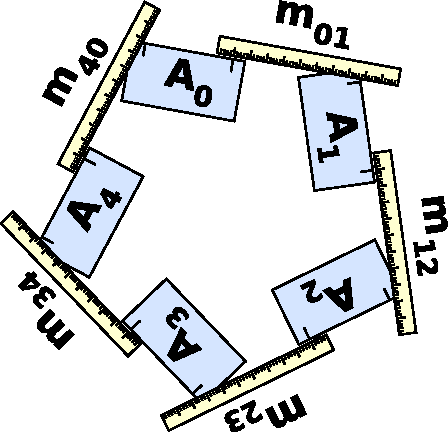
\includegraphics[width=0.37\linewidth]{PLOTS/propagating_example2.pdf}
\end{center}
\end{minipage}

\vspace{0.4 cm}
In this case, the measurements are not a linear distance but either an
angle $\phi$ or an $r\phi$ displacement along an arc of constant
radius $r$.  This is a common configuration in particle physics, as
tracking detectors are often built to encircle a beamline and
collision point.  Figure~\ref{fig:beamhalo_ring} shows an example from
muon endcap alignment.

\begin{figure}
\begin{center}
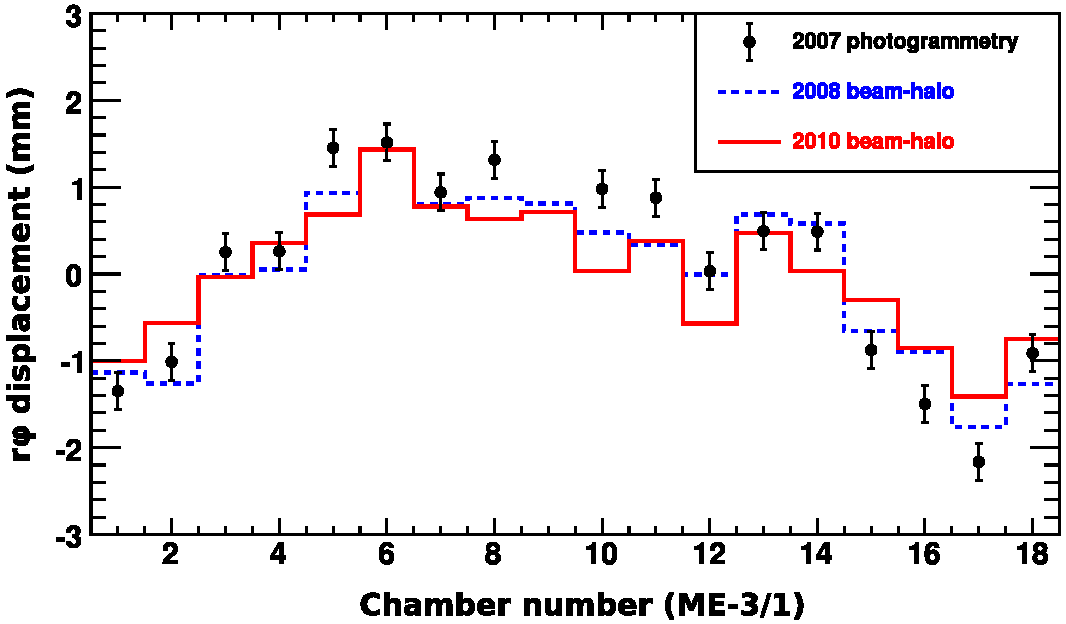
\includegraphics[width=0.75\linewidth]{PLOTS/compare_m31_x.pdf}
\end{center}
\caption{Beam-halo alignment measurements propagated around a circular
  ring as in Eq.~\ref{eqn:propagating_example3} and photogrammetry
  (direct measurements relative to a single coordinate frame origin).
  The vertical axis is $A_i$ expressed relative to a design
  configuration, and the horizontal axis is
  $i$. \label{fig:beamhalo_ring}}
\end{figure}

Given the symmetry of the problem, we may want to chose a more
symmetric coordinate system constraint than $A_0 = 0$.  Fixing the
average of all alignment corrections, $\sum_i A_i = 0$ (or any other
subset), solves the same problem.  The numerical results differ only
in a shift of the overall coordinate system.

\subsection{General Alignment Fit}

\begin{minipage}{\linewidth}
In general, $N_a$ alignables $A_i$ are constrained by $N_m$
measurements $m_{ij}$, where measurements can relate any two
alignables.  If we interpret the $A_i$ as nodes and the $m_{ij}$ as
edges of a graph, we can draw a ``constraint diagram'' to represent
the system.  The two cases we have studied so far are
\begin{center}
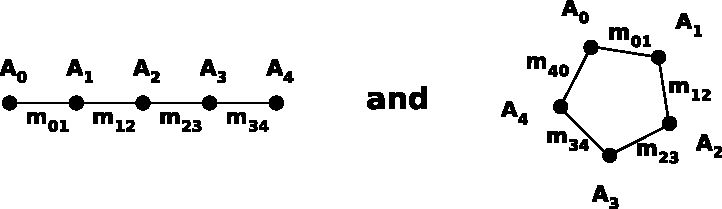
\includegraphics[width=0.75\linewidth]{PLOTS/two_diagrams.pdf}
\end{center}
\end{minipage}
The constraint diagram, measurement uncertainties, and choice of
coordinate system completely determine the matrix that needs to be
inverted to solve a given alignment problem.

The objective function for a general one-dimensional alignment
(centered on a subset of alignables $S \subseteq [0, N_a)$) is
\begin{equation}
\chi^2 = \sum_{i=0}^{N_a} \sum_{j=0}^{N_a}
\left(q_{ij} \frac{m_{ij} - A_i + A_j}{\sigma_{ij}}\right)^2
+ \lambda \left(\sum_{i \in S} A_i \right)^2
\label{eqn:general_chi2}
\end{equation}
where $q_{ij} = 1$ if a measurement exists and $0$ if it does not
exist.  (We could have introduced fewer variables by saying that there
is an edge between every two nodes and allowing some of them to have
$1/\sigma_{ij} = 0$, but we don't usually think of unmeasured
parameters as being ``measured with infinite uncertainty.'')  The
alignment solution is obtained when $A_i$ are chosen such that
$\chi^2$ is minimized.  The values of $A_i$ may be ``absolute'' or
``relative,'' where ``absolute'' means that each $A_i$ is the distance
between an alignable and a common origin, while ``relative'' means
that an initial configuration is assumed (the ``prior geometry'') with
$m_{ij}$ being measurements that would be zero if the prior geometry
were correct, and $A_i$ are the changes needed to make the alignment
correct.  The latter is more useful for track-based alignment, because
it is necessary to assume an initial alignment to fit tracks.

The last term in Eq.~\ref{eqn:general_chi2} is a Lagrange multiplier
to enforce a coordinate system in which the average of $A_i$ for $i
\in S$ is zero.  Any coordinate system could be chosen, and changes in
$A_i$ change the coordinate system--- a fact which must be considered
when comparing two alignment solutions.

Since Eq.~\ref{eqn:general_chi2} is quadratic in all $A_i$, its first
derivatives are linear, so the minimum can be calculated by setting
the first derivatives to zero and solving the system.  The matrix that
is used to solve the system of first derivatives is the matrix of
second derivatives (the ``Hessian'').  With the following definitions,
\begin{eqnarray}
v_k &=& \sum_{i=0}^{N_a} \frac{m_{ik}}{{\sigma_{ik}}^2} - \sum_{j=0}^{N_a} \frac{m_{kj}}{{\sigma_{kj}}^2} \\
M_{kl} = \frac{\partial^2 \chi^2}{\partial A_k \partial A_l} &=& \delta_{kl} \left(\sum_{i=0}^{N_a} \frac{q_{ik}}{{\sigma_{ik}}^2} + \sum_{j=0}^{N_a} \frac{q_{kj}}{{\sigma_{kj}}^2} \right) - \frac{q_{kl}}{{\sigma_{kl}}^2} - \frac{q_{lk}}{{\sigma_{lk}}^2}
+ \sum_{i \in S} \lambda,
\label{eqn:v_m_definitions}
\end{eqnarray}
the $\vec{A}$ (vector of $A_i$) that minimizes $\chi^2$ is
\begin{equation}
\vec{v} = M \cdot \vec{A} \mbox{ or } \fbox{$\vec{A} = M^{-1} \cdot \vec{v}$.}
\label{eqn:general_solution}
\end{equation}

To get a feeling of how this works, try executing the following Python
program.  It sets up a ring of alignment measurements and solves the
system (a)~by minimizing Eq.~\ref{eqn:general_chi2} with the general
minimization package Minuit, and (b)~by solving the linear system of
Eq.~\ref{eqn:v_m_definitions}--\ref{eqn:general_solution}.

\begin{python}
# some definitions
lam = 1e8     # lambda (Lagrange multiplier in Eq. 14)
Na = 5        # number of alignables A_i
fixed = None  # if fixed is None, S = [0, Na) (fix the average of all)
              # if fixed is a number, S = [fixed] (fix one alignable)

# representation of the measurements m_ij
class Measurement:
    def __init__(self, i, j, value, error):
        self.i, self.j, self.value, self.error = i, j, value, error

measurements = [
    Measurement(0, 1,  0.12, 0.01),
    Measurement(1, 2,  0.00, 0.01),
    Measurement(2, 3, -0.15, 0.01),
    Measurement(3, 4, -0.15, 0.01),
    Measurement(4, 0,  0.18, 0.01),
    ]
Nm = len(measurements)   # number of measurements m_ij

# objective function (Eq. 14) with an arbitrary number of arguments
def chi2_arbitrary(*args):
    if fixed is None: s = lam * sum(args)**2
    else: s = lam * args[fixed]**2
    for m in measurements:
        s += (m.value - args[m.i] + args[m.j])**2 / m.error**2
    return s
# put it in a form that Minuit accepts (specific number of arguments)
chi2_arguments = ", ".join(["A%i" % i for i in range(Na)])
chi2 = eval("lambda %s: chi2_arbitrary(%s)" %
            (chi2_arguments, chi2_arguments))

# (a) minimize the objective function using Minuit
import minuit
minimizer = minuit.Minuit(chi2)
minimizer.migrad()
print "Minuit", [minimizer.values["A%i" % i] for i in range(Na)]

# (b) minimize the objective function using linear algebra
from numpy import matrix
from numpy.linalg.linalg import inv, dot

# Equation 15
def vk(k):
    s = 0.
    for m in measurements:
        d = 1.*m.value/m.error**2
        if m.i == k: s += d
        if m.j == k: s -= d
    return s
v = [vk(k) for k in range(Na)]

# Equation 16
def Mkl(k, l):
    if fixed is None: s = lam
    else:
        if k == 0 and l == 0: s = lam
        else: s = 0.
    for m in measurements:
        d = 1./m.error**2
        if k == l and (m.i == k or m.j == k):
            s += d
        if (m.i == k and m.j == l) or (m.j == k and m.i == l):
            s -= d
    return s
M = matrix([[Mkl(k, l) for k in range(Na)] for l in range(Na)])

# Equation 17
print "Linear algebra", dot(inv(M), v)
\end{python}

The output should be
\begin{python}
Minuit [0.0060000000945981046, -0.11399999990522246, -0.11399999990562885, 
                                0.036000000094937618, 0.18600000009519196]
Linear algebra [[ 0.006 -0.114 -0.114  0.036  0.186]]
\end{python}
The Minuit and algebraic results are nearly the same: Minuit searches
$\chi^2(A_0, A_1, A_2, A_3, A_4)$ for a minimum and stops when it gets
within a certain tolerance, while the matrix inversion finds the exact
minimum in one step.  Note that the Minuit minimization only accesses
$\chi^2$ while the algebraic solution only accesses $v_k$ and
$M_{kl}$, so comparing the two verifies that the derivatives were
properly calculated.

To see uncertainties in the alignment (covariance matrices), implement
the following function in your Python script:
\begin{python}
def print_matrix(mat):
    if not isinstance(mat, dict):  # put all matrices in the same format
        m = {}
        for i in range(Na):
            for j in range(Na):
                m["A%d" % i, "A%d" % j] = mat[i, j]
    else:
        m = mat
    # pretty-print matrices which are in that format
    print "\n".join([" ".join(["%8.2g" % m["A%d" % i, "A%d" % j]
                               for j in range(Na)]) for i in range(Na)])
\end{python}
and print Minuit's covariance matrix and $M^{-1}$.
\begin{python}
>>> print_matrix(minimizer.covariance)  # Minuit
   4e-05  5.7e-10   -2e-05   -2e-05  2.5e-10
 5.7e-10    4e-05  3.1e-10   -2e-05   -2e-05
  -2e-05  3.1e-10    4e-05    4e-10   -2e-05
  -2e-05   -2e-05    4e-10    4e-05  5.1e-10
 2.5e-10   -2e-05   -2e-05  5.1e-10    4e-05

>>> print_matrix(inv(M))  # Linear algebra
   4e-05    4e-10   -2e-05   -2e-05    4e-10
   4e-10    4e-05    4e-10   -2e-05   -2e-05
  -2e-05    4e-10    4e-05    4e-10   -2e-05
  -2e-05   -2e-05    4e-10    4e-05    4e-10
   4e-10   -2e-05   -2e-05    4e-10    4e-05
\end{python}
Again, Minuit provides an approximation to the matrix solution: only
the smallest elements of the result differ.

As an exercise, try changing the collection of fixed alignables $S$,
so that the minimization holds $A_0$ fixed, or $A_1$, etc.  Are the
results equivalent under global translation?  Try changing the
measurement constraints and their uncertainties: do the results make
sense?  Try to encode the constraint diagram in
Fig.~\ref{fig:twelve_alignables} as a list of measurements
(measurements $m_{ij}$ are the numbers marked on the edges; assume all
$\sigma_{ij}$ are 0.01).

\begin{figure}
\begin{center}
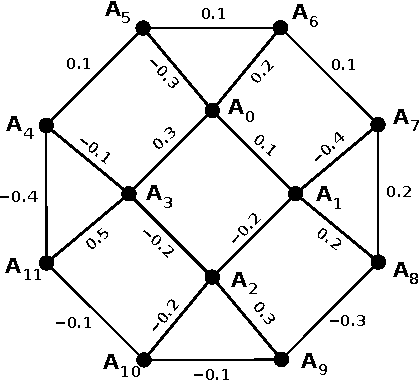
\includegraphics[width=0.5\linewidth]{PLOTS/toy_example.pdf}
\end{center}
\caption{Constraint diagram used in several examples.  Nodes are
  labeled alignables $A_i$ and the values on the edges represent
  $m_{ij}$. \label{fig:twelve_alignables}}
\end{figure}

Do you get the following result?
\begin{python}
>>> print dot(inv(M), v)
[[ 0.01791667 -0.12458333  0.02791667  0.14541667  0.22625    -0.07625
  -0.17291667 -0.26041667 -0.18375     0.13375     0.05708333  0.20958333]]
\end{python}
Remember that this is still a one-dimensional example; the graph
simply depicts which alignables are measured relative to which others.

\subsection{Error Analysis}

We have already seen how independent alignment measurements $m_{ij}$
can be propagated to a final covariance matrix on $A_i$, but the
covariance matrix doesn't give an intuitive sense of the uncertainties
because it is far from being diagonal.  This section shows how the
uncertainties can be transformed to a more meaningful form.

We can recast the alignment solution (Eq.~\ref{eqn:general_solution}), 
\begin{equation}
\vec{A} = M^{-1} \cdot \vec{v} \hspace{0.25 cm} \pm \hspace{0.25 cm} M^{-1},
\label{eqn:thesolutionagain}
\end{equation}
in a different basis in which the transformed $A_i$ have linearly
independent uncertainties.  Suppose that $B$ is a matrix such that
$B^{-1} M^{-1} B$ is diagonal.  By left-multiplying
Eq.~\ref{eqn:thesolutionagain} by $B^{-1}$ and inserting an identity,
\begin{equation}
B^{-1} \vec{A} = \left( B^{-1} M^{-1} B \right) \cdot B^{-1} \vec{v}.
\end{equation}
The vector $B^{-1} \vec{A}$ presents the same solution in different
coordinates: linear combinations of the actual alignable positions,
and by analogy with Eq.~\ref{eqn:thesolutionagain}, the uncertainty in
these coordinates is $B^{-1} M^{-1} B$, a diagonal covariance matrix.
Therefore, the $B^{-1} \vec{A}$ coordinates are statistically
independent of each other.  Let's call these the ``modes'' of the
alignment.





%% Combining alignment measurements into a consistent system:
%% motivating examples, solution space is not $R^N$ ("gauge
%% invariance"), logic and formalism of simultaneous fitting with
%% "constraint diagrams", Hessian, and working toy example scripts.
%% Overconstrained systems and closure tests.  Error analysis:
%% decomposition of statistical errors into weak and strong modes,
%% characterization of the undetermined and weakest modes, systematic
%% errors in measurements.

\section{Measuring Detector Positions with Tracks}
\label{sec:measuring_detector_positions_with_tracks}

%% Alignment measurements from tracks: 6-DOF rigid body parameter
%% space, track residuals space including the 4 relevant track
%% parameters, and the differential map (2dresid, 3doflargestruct,
%% 6dof, 5dof, 6dofrphi) between them (linearization and iteration),
%% significance of the chamber origin, simple studies using elements
%% of the map, example from CRUZET alignment, toy example in pyROOT
%% (linear fit to plot and transformed residuals), full
%% track-parameter/alignment-parameter correlations and their
%% solutions: large-scale iteration and Millepede, Reference-Target
%% factorization of the problem.

\section{Realistic Tracking and Diagnostics of Track-Bias}
\label{sec:realistic_tracking_and_diagnostics_of_track_bias}

%% Systematic errors in realistic tracking: magnetic field errors,
%% material budget errors, and the q/pT, q/pz plots, Rutherford and
%% multiple scattering, argument for fitting to the peak, rather than
%% mean (CRUZET example), extension of the objective function and
%% non-linear minimization (PyMinuit example), cross-checks of
%% redundant constraints in the differential map, diagnosing track
%% biases: discontinuities at chamber boundaries (map plots),
%% differences of residuals on the same track (segment-difference
%% plots), and scaling of phi, theta, and curvature bias scaling with
%% pathlength.

\section{CSCOverlapsAlignmentAlgorithm: a Complete Alignment Package}
\label{sec:cscoverlapsalignmentalgorithm_a_complete_alignment_package}

\section{Conclusion}
\label{sec:conclusion}

%% Closing, where to find more information

\appendixpage
\appendix
\section{Summarizing Datasets with Running Sums}
\label{sec:summarizing_datasets_with_running_sums}

It is often necessary to reduce a dataset to a few numbers by
computing its mean or by fitting it to a straight line.  There are
many ways to do this, but the least intrusive method (no external
packages) with the smallest memory usage is with running sums.
Several quantities are initialized to zero, incremented in a loop over
the data, and the desired quantities are calculated from the running
sums at the end of the loop.  These kinds of calculations are
ubiquitous in alignment code, but easy to get slightly wrong, so it's
good practice to check.

\subsection{Mean and Weighted Mean}

The mean is simply a weighted mean with all weights equal to 1.  The
uncertainty in the weighted mean ({\tt weighted\_mean\_err}) does not
reflect the width of the distribution, only the uncertainties given by
the dataset ({\tt xerr}).

\vspace{0.6 cm}
\begin{tabular}{p{0.4\linewidth} p{0.6\linewidth}}
{\bf Mean} & {\bf Weighted mean} \\
\begin{python}
sum_1 = 0.
sum_y = 0.
for y in data:
    sum_1 += 1.
    sum_y += y
if sum_1 != 0.:
    mean = sum_y / sum_1
else: raise Exception
\end{python} &
\begin{python}
from math import sqrt
sum_1 = 0.
sum_y = 0.
for y, yerr in data:
    weight = 1./yerr**2
    sum_1 += weight
    sum_y += weight * y
if sum_1 != 0.:
    weighted_mean = sum_y / sum_1
    weighted_mean_err = sqrt(1./sum_1)
else: raise Exception
\end{python}
\end{tabular}

\subsection{Linear fitting}

A linear fit is an extension of the weighted mean to account for a
trend in the data as a function of an independent coordinate {\tt x}.
Sometimes knowing the slope is useful in itself, but sometimes a
linear fit is needed only to remove the effect of non-uniformity in
the {\tt x} distribution.  For example, suppose that a dataset is
non-uniformly distributed in {\tt x} and also has a linear trend in
{\tt y} vs.\ {\tt x}.  The fitted intercept quantifies the typical
{\tt y} value at {\tt x=0}, but the mean of {\tt y} does not.

\begin{center}
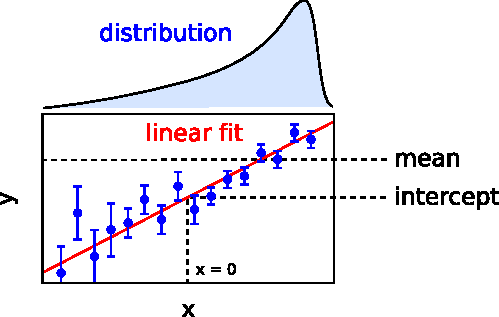
\includegraphics[width=0.5\linewidth]{PLOTS/nonuniform_explanation.pdf}
\end{center}

\begin{python}
from math import sqrt
sum_1 = 0.
sum_x = 0.
sum_xx = 0.
sum_y = 0.
sum_xy = 0.
for x, y, yerr in data:
    weight = 1./yerr**2
    sum_1 += weight
    sum_x += weight * x
    sum_xx += weight * x**2
    sum_y += weight * y
    sum_xy += weight * x * y
delta = (sum_1 * sum_xx) - (sum_x * sum_x)
if delta != 0.:
    intercept = ((sum_xx * sum_y) - (sum_x * sum_xy)) / delta
    intercept_err = sqrt(sum_xx / delta)

    slope = ((sum_1 * sum_xy) - (sum_x * sum_y)) / delta
    slope_err = sqrt(sum_1 / delta)

else: raise Exception
\end{python}

\subsection{Root-mean-square and Standard Deviation}

The root-mean-square (RMS) characterizes both the width of a
distribution and its deviation from zero, while the standard deviation
(stdev) only characterizes the width of the distribution.  Note that
$\mbox{\tt rms}^2 = \mbox{\tt stdev}^2 + \mbox{\tt mean}^2$.

\vspace{0.6 cm}
\begin{tabular}{p{0.45\linewidth} p{0.55\linewidth}}
{\bf Root-mean-square (RMS)} & {\bf Standard deviation (stdev)} \\
\begin{python}
from math import sqrt
sum_1 = 0.
sum_yy = 0.
for y in data:
    sum_1 += 1.
    sum_yy += y**2
if sum_1 != 0.:
    rms = sqrt(sum_yy / sum_1)
else: raise Exception
\end{python} &
\begin{python}
from math import sqrt
sum_1 = 0.
sum_y = 0.
sum_yy = 0.
for y in data:
    sum_1 += 1.
    sum_y += y
    sum_yy += y**2
if sum_1 != 0. and (sum_yy / sum_1) > (sum_y / sum_1)**2:
    stdev = sqrt((sum_yy / sum_1) -
                 (sum_y / sum_1)**2)
else: raise Exception
\end{python}
\end{tabular}

The stdev may be used instead of a dataset's given uncertainties ({\tt
  yerr}) to quantify the uncertainty in the mean.  This implicitly
assumes that the width of the distribution is due to statistical
uncertainty, rather than an unnoticed trend.  The uncertainty in the
mean is $\sqrt{\mbox{\tt stdev} / \mbox{\tt sum\_1}}$ and the
uncertainty in the RMS and stdev are $\sqrt{\mbox{\tt stdev} / (2 \cdot
  \mbox{\tt sum\_1})}$.

\subsection{Covariance and Correlation}

The covariance of a distribution is an extension of the stdev in two
(or more) dimensions, quantifying the off-diagonal elements in a
covariance matrix
\begin{equation}
\sigma = \left(\begin{array}{c c}
\sigma_{xx} & \sigma_{xy} \\
\sigma_{xy} & \sigma_{yy}
\end{array}\right)
\end{equation}
where $\sqrt{\sigma_{xx}}$ and $\sqrt{\sigma_{yy}}$ are the stdev of the
{\tt x} and {\tt y} distributions, respectively, and $\sigma_{xy}$
is the covariance.  Correlation is the same thing, normalized such
that diagonal elements are 1 (quantifies only the shape of the error
ellipse).

\vspace{0.6 cm}
\begin{tabular}{p{0.45\linewidth} p{0.55\linewidth}}
{\bf Covariance} & {\bf Correlation} \\
\begin{python}
def mean(data):
    return sum(data)/len(data)
xmean = mean(xdata)
ymean = mean(ydata)

sum_xy = 0.
for x, y in zip(xdata, ydata):
    sum_xy += (x - xmean) *
              (y - ymean)
covariance = sum_xy/len(data)
\end{python} &
\begin{python}
from math import sqrt
def mean(data):
    return sum(data)/len(data)
xmean = mean(xdata)
ymean = mean(ydata)

sum_xx = 0.
sum_yy = 0.
sum_xy = 0.
for x, y in zip(xdata, ydata):
    sum_xx += (x - xmean)**2
    sum_yy += (y - ymean)**2
    sum_xy += (x - xmean) *
              (y - ymean)
if sum_xx * sum_yy != 0.:
    correlation = sum_xy /
            sqrt(sum_xx * sum_yy)
else: raise Exception
\end{python}
\end{tabular}

\end{document}
